\documentclass[12pt, dutch]{article}
\usepackage{hyperref}
\usepackage{graphicx}
\usepackage{subcaption}
\hypersetup{
    colorlinks=true,
    linkcolor=black,
    filecolor=magenta,      
    urlcolor=blue,
    pdfpagemode=FullScreen,
    }
\urlstyle{same}
\title{HEAP1: basisoperaties in binaire max heaps}
\author{Manoah Kinnaert}
\graphicspath{{charts/HEAP1}}
\begin{document}

\begin{titlepage}
    \maketitle
\end{titlepage}
\pagebreak
\section{Korte inleiding}
In dit (korte) verslag bespreken we een experiment rond binaire max heaps. We bekijken de kost in exchanges en compares voor de elementaire sink en swim operaties 
bij het toevoegen van elementen in heaps, alsook bij het verwijderen van het grootste element uit een heap.
Alle code die gebruikt is voor dit experiment is hier terug te vinden: \\\ 
\url{https://github.com/ManoahKinnaert/HEAP}.

\section{Verloop van de experimenten}
In dit experiment nemen we n voor het aantal elementen die zich in de heap bevinden.  
Voor de inserts in de heap doen we het experiment op twee manieren.
Voor het eerste doen we het door te vertrekken van een lege array en telkens een element toe te voegen en deze dan te laten zakken in de heap.
Deze elementen die toegevoegd worden zijn random en worden gegenereerd met een uniforme verdelings functie uit de standard library van Python.
De heap wordt dus telkens groter en groter. We verwachten hier hoogstens \begin{math} 1 + \lfloor \log_2 n \rfloor \end{math} compares.
En voor het aantal exchanges verwachten we hoogstens \begin{math} \lfloor \log_2 n \rfloor \end{math} exchanges.

Voor het tweede vertrekken we van een array van uniform verdeelde random getallen en heapifyen we de array. 
Door te beginnen met het laatste element dat kinderen heeft en deze elementen te laten 'zinken'. Dit doen we van dit laatste element 
tot en met het 'wortelelement'. Voor het aantal compares in functie van n verwachten we hier hoogstens \begin{math} 2n\end{math} compares.
En voor het aantal exchanges verwachten we hoogstens \begin{math} n \end{math} exchanges.

Voor het verwijderen van de grootste waarde in de heap is het experiment eenvoudiger.
We bouwen eerst een heap op van grootte n en verwijderen dan systematisch het grootste element oftewel het 'wortelelement'.
Iedere keer dat we het 'wortelelement' verwijderen tellen we het aantal compares en exchanges.
Voor de compares verwachten we hier hoogstens \begin{math} 2\lfloor \log_2 n \rfloor \end{math} compares. En voor het aantal exchanges 
verwachten we hoogstens \begin{math} 1 + \lfloor \log_2 n \rfloor \end{math} exchanges.

\section{Bevindingen plotten}
Voor het plotten van het aantal compares en exchanges bij het toevoegen van elementen is er voor de 'eerste manier' gebruik gemaakt van 
een logaritmische y-as. We verachtten immers logaritmisch gedrag dus waarom niet\dots
Voor alle andere grafieken is er gebruik gemaakt van een normale lineaire schaal voor de assen.

\section{Bevindingen}
Voor de experimenten rond het toevoegen van elementen aan een heap zien we dat het aantal compares en exchanges duidelijk onder de theoretische bovengrenzen blijft. De gemeten waarden benaderen de theoretische curves wel, maar overschrijden deze niet.
Dit resultaat is verwacht, aangezien de theoretische curves een worst-case analyse weergeven. In praktijk zullen inserts vaak minder swaps en vergelijkingen vereisen, afhankelijk van de ingevoegde waarden en de reeds opgebouwde heapstructuur.
De resultaten bevestigen dus dat de implementatie van de heap-operaties correct gedrag vertoont en binnen de theoretische complexiteitsgrenzen blijft.

In de resultaten zit ook goed nieuws aangezien wordt waargenomen dat het worst-case aantal compares en exchanges niet vaak wordt gehaald bij het toevoegen van random elementen.
Ook het verwijderen van de grootste elementen uit de heapstructuren die met random elementen zijn opgebouwd zien we vergelijkbaar gedrag.
De theoretische bovengrenzen worden in de praktijk dus zelden benaderd (zie grafieken op volgende bladzijde).

\begin{figure}[htbp]
    \centering
    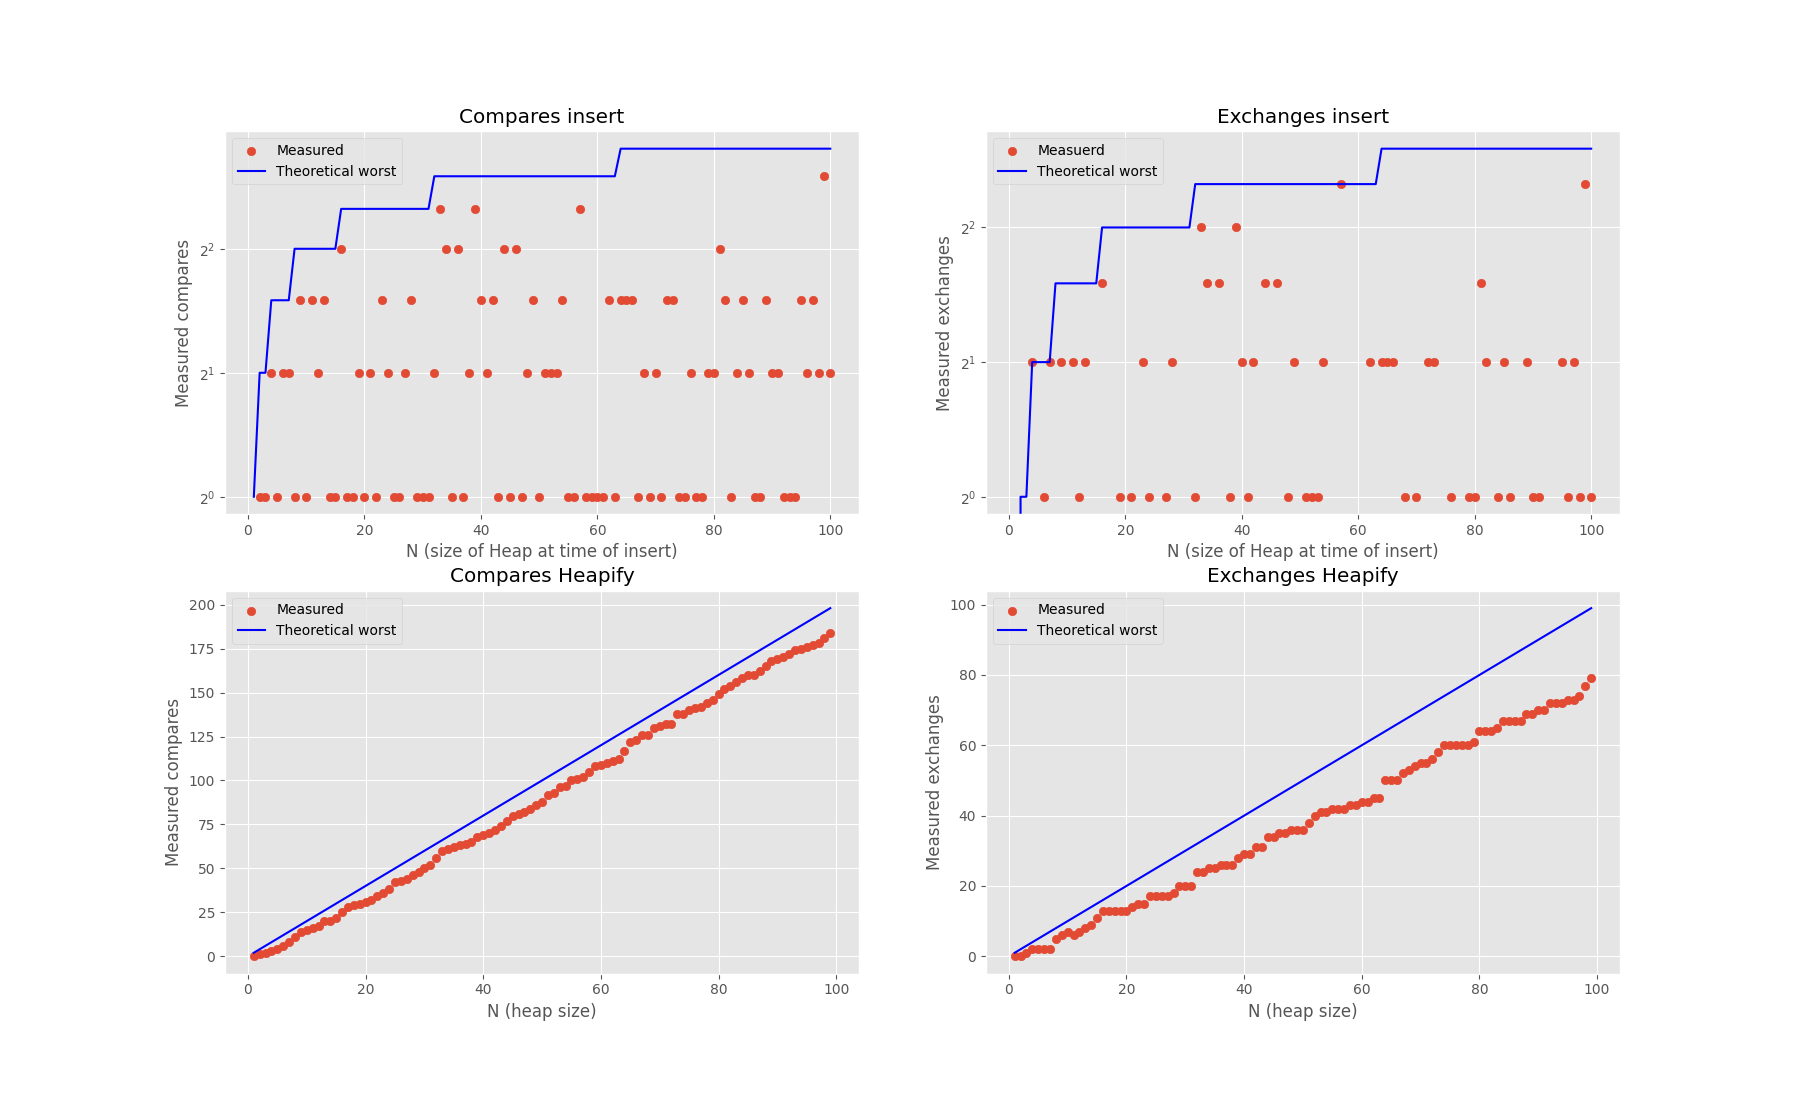
\includegraphics[width=0.9\textwidth]{Figure_1.png}
    \caption{Heap insert (indien niet duidelijk genoeg zie git repo)}
    \label{fig:heap_insert_1}
    \vspace{0.8cm}
    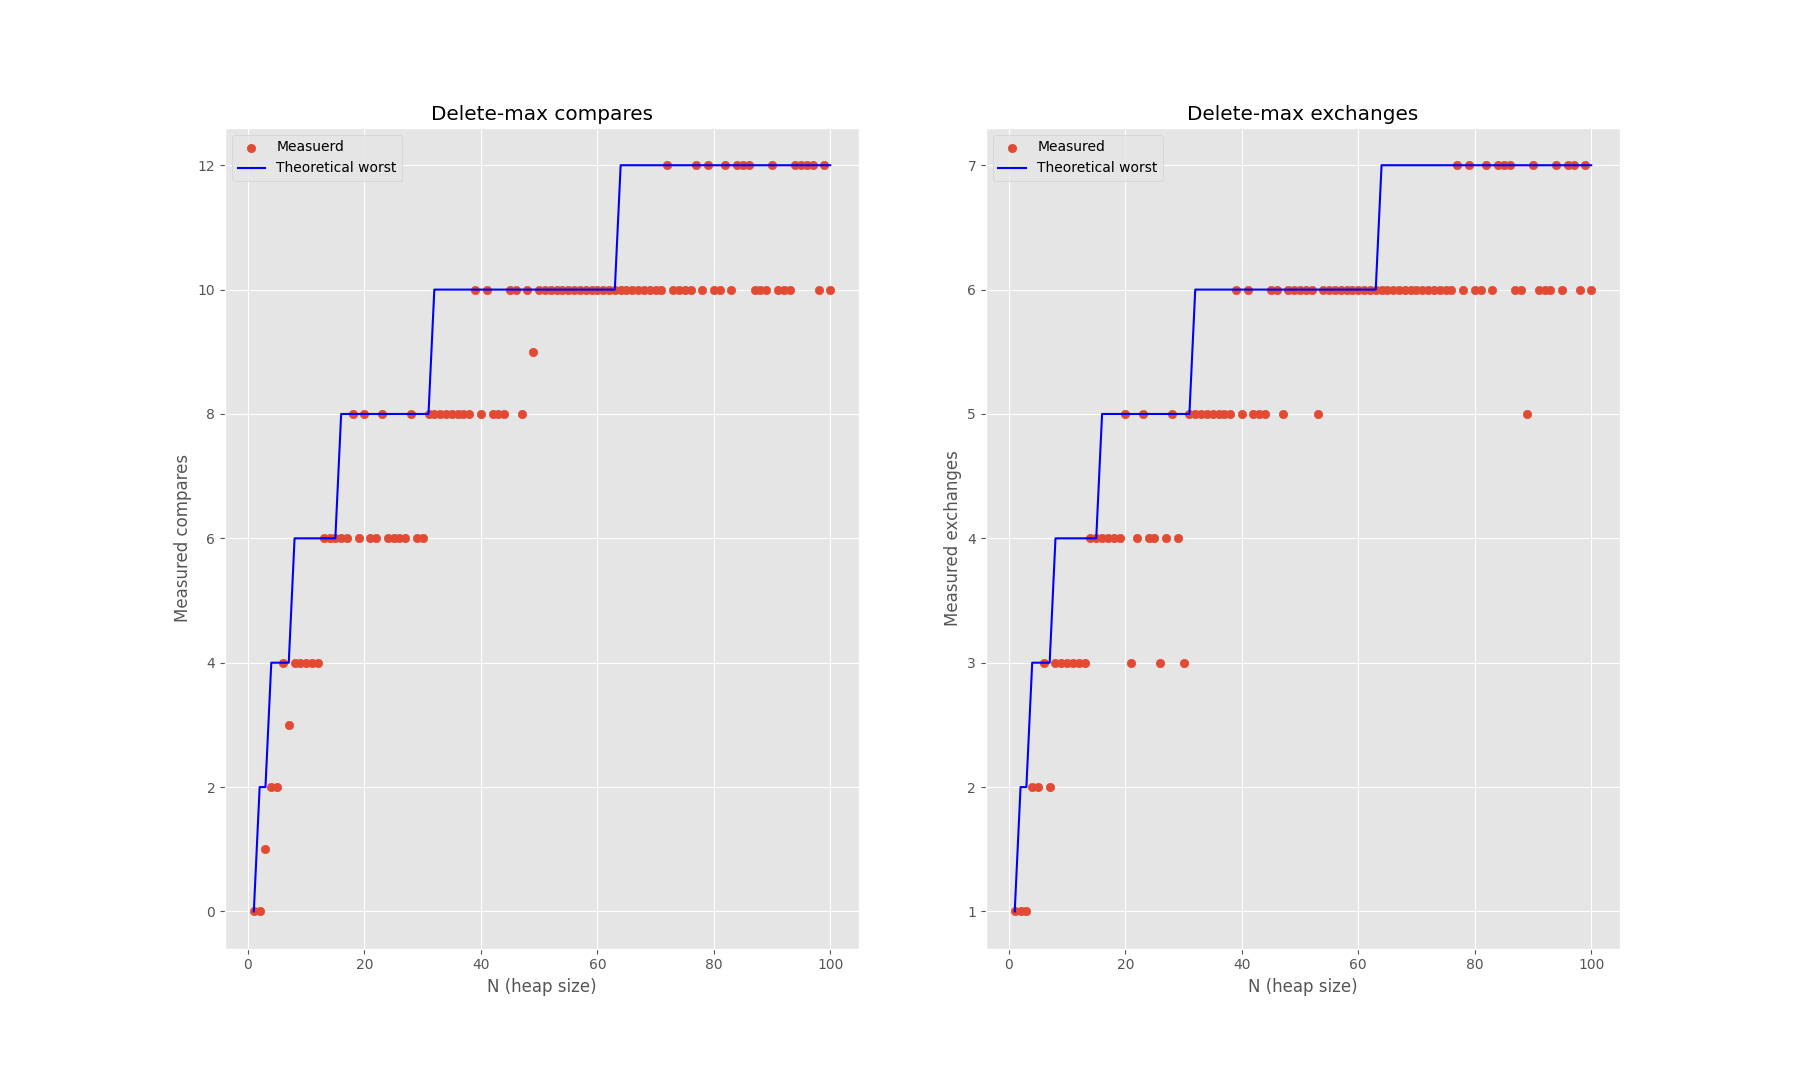
\includegraphics[width=0.9\textwidth]{Figure_2.png}
    \caption{Heap delete max (indien niet duidelijk genoeg zie git repo)}
    \label{fig:heap_insert_2}
\end{figure}

\end{document}